\documentclass[11pt,a4paper]{article}

\usepackage{main}
\usepackage{evaluation}

\renewcommand{\typedocument}{Évaluation}
\renewcommand{\classe}{6e}
\renewcommand{\titre}{Évaluation 2 -- Mouvement (Sujet B)}

\begin{document}

\creertitre{\titre}

\begin{center}
\textit{Durée : 45 minutes -- Calculatrice autorisée \\ Tous les exercices sont à faire sur la copie.}
\end{center}

\exercice[6]{Questions de cours}

\question[2]{Rappeler la définition d'un référentiel.}

\question[2]{Comment appelle-t-on un mouvement dont la trajectoire est un cercle ?}

\question[2]{Que peut-on dire sur la vitesse d'un mouvement accéléré ?}

\exercice[6]{Référentiels}

\begin{center}
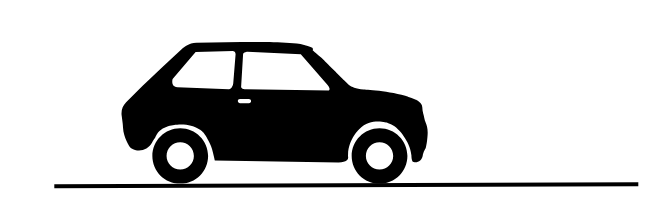
\includegraphics[width=0.5\textwidth]{images/voiture.png}
\end{center}

Félix est assis dans une voiture. La voiture roule en ligne droite avec une vitesse constante.

\question[1.5]{Est-ce que Félix est en mouvement par rapport à la voiture ?}
\question[1.5]{Est-ce que Félix est en mouvement par rapport au sol ?}
\question[3]{Décrire le mouvement de Félix par rapport au sol avec deux adjectifs du cours.}

\exercice[8]{Vitesse}

\question[1]{Rappeler la formule de la vitesse, avec les noms des grandeurs physiques.}

\question[1]{Quelles sont les deux unités possibles pour la vitesse ?}

\question[6]{Répondez aux questions suivantes en détaillant vos calculs et en justifiant vos réponses.}

\begin{enumerate}[label=\alph*)]
    \item Les tigres les plus rapides peuvent atteindre une vitesse de \SI{20}{\meter/\second}. A cette vitesse, quelle distance peuvent-ils courir en 7 secondes ?\\[0.2em]
    \item Un avion de chasse peut parcourir \SI{30000}{\meter} en 1 minute. Quelle est sa vitesse moyenne en m/s ?\\[0.2em]
    \item Un train à grande vitesse (TGV) à destination de Strasbourg part de Paris à 10h00. La distance entre Paris et Strasbourg est de 400 km. Si sa vitesse moyenne est de 200 km/h, combien de temps durera le trajet ? À quelle heure arrivera le train à Strasbourg ?
\end{enumerate}

\end{document}